\documentclass[a4paper]{article}

\usepackage[T1]{fontenc}
\usepackage[english]{babel}

\usepackage{hyperref}
\hypersetup{%
    pdfauthor = {Tobias Andersson, Victor Koronen},
    pdftitle = {ID1217: The Green Elevator},
    pdfsubject = {ID1217},
    pdfkeywords = {parallel programming},
    pdfcreator = {LaTeX with hyperref package},
    pdfproducer = {pdflatex}
}

\usepackage{graphicx}

\title{ID1217: ``The Green Elevator''}
\author{%
    Tobias Andersson <\href{mailto:tobias2@kth.se}{tobias2@kth.se}> \and
    Victor Koronen <\href{mailto:koronen@kth.se}{koronen@kth.se}>
}
\date{\today}

\begin{document}

\maketitle
\thispagestyle{empty}

\section{Introduction}

Our task was to design, implement and evaluate a controller for a simulated set
of elevators, see figure \ref{fig:hardware_control_panel}.

\begin{figure}[p]
    \centering
    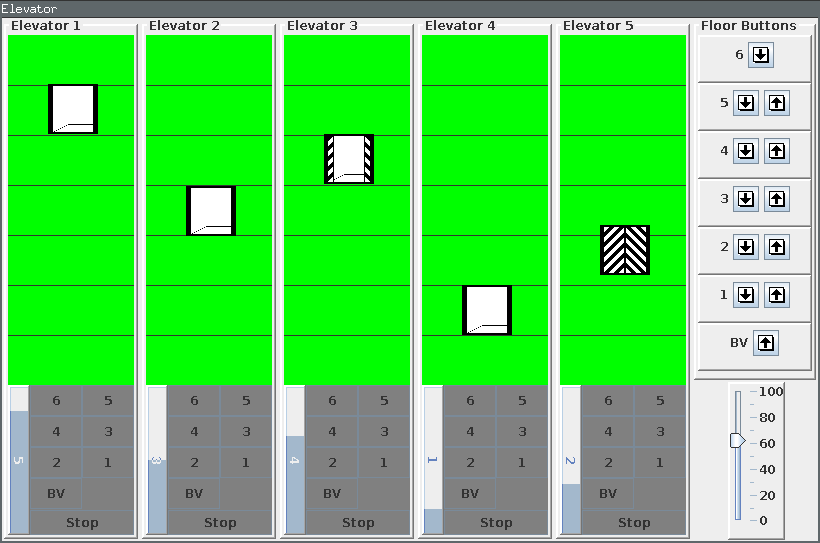
\includegraphics[width=1.0\textwidth]{images/elevators_5_6.png}
    \caption{The hardware control panel.}
    \label{fig:hardware_control_panel}
\end{figure}

\section{Implementation}

We decided to implement the controller application in Java, since it is a
language we both felt comfortable with. This also allowed us to utilize classes
from the extensive Java Standard Library and to develop the program using the
Eclipse IDE. We mainly developed the controller application in our laptops,
which both run a recent edition of the GNU/Linux Ubuntu OS.

\subsection{Structure}

The controller application consists of a set of classes with different
responsibilities. Some of the important classes are described briefly below. For
a more detailed description, see the corresponding JavaDoc.

% Describe your implementation (functions, classes, interfaces).
\begin{description}

\item[\texttt{Main}] The main entry point to the controller program. Parses
    command line parameters, sets up the network connection and passes control
    over to \texttt{MasterController}.

\item[\texttt{MasterController}] Receives messages from the hardware. Decides
    which elevator should respond to floor button presses and passes cabin
    button presses onto an instance of \texttt{ElevatorController}.

\item[\texttt{ElevatorController}] The control unit for one of the elevators.
    Each elevator has a separate instance of this class. Manages the route for
    this elevator and controls the motors. This class contains most of the
    important logic.

\item[\texttt{SocketHardwareController}] The main component of our port of the C
    hardware API. Handles communication with the hardware via a TCP socket.

\end{description}

\subsection{Algorithms}
% Describe algorithms you have developed (chosen), synchronization or/and
% communication mechanisms you have used, and explain motivation for your design
% choices.
In this section, important algorithms used in the project are described. More
specifically the way an elevator is chosen to service a floor button press and
the way an individual elevator is controlled, followed by synchronization
mechanisms used.

\subsubsection{Choosing an elevator}

As mentioned above, the \texttt{MasterController} class is responsible for
choosing which elevator will service a floor button press. This is done by using
a heuristic for determining the cost for an elevator to service a request based
on the nature of the request and the elevator's current state. This cost
function is located in the \texttt{ElevatorController} class. When the
\texttt{MasterController} receives a request it calls the cost function of each
\texttt{ElevatorController} and assigns the task to the elevator with the least
cost by adding it to the end of that elevator's command queue.

The cost of a request starts at $0$ and based on the request and the state of
the elevator, costs are added and subtracted in the following manner.

\begin{itemize}
\item A cost of $1500$ is subtracted from elevators that are currently stationary
    at the requested floor without any pending commands in their queue.
\item A cost of $10$ is added to elevators that are currently active. This is
    because elevators that are not active can begin to serve the request
    immediately, which may reduce waiting time.
\item A cost of $5$ is added to elevators that are currently active and are
    moving away from the floor where the request was made. This is because the
    elevator will need to turn after it has finished its current task, which
    mean that waiting time will probably be long.
\item A cost of $15$ is subtracted if the request can be processed along the
    way, for instance if an elevator is heading upwards and the up-button is
    pressed on a floor that the elevator will pass before changing direction.
\item Finally a cost equal to the distance from the elevator to the desired
    floor is added. This is to make it so the closest elevator is always chosen,
    should there be multiple options.
\end{itemize}

\subsubsection{Controlling an elevator}

Each elevator is controlled by an instance of the \texttt{ElevatorController}
class. Each \texttt{ElevatorController} has a queue of tasks that have been
assigned to it. This includes all button presses made inside the cabin and all
floor button presses which has been assigned to it by the master controller.

The elevator controller performs tasks by looking at the first item in the queue
and then starts to process that task without removing it from the queue.
Processing a task means closing the doors if needed and then starting the motors
in the direction of the requested floor. Then the controller will repeatedly
sleep and poll the elevator's position and update the scale. If the elevator is
at a floor and that floor is in the queue of commands, the elevator will stop
and remove that command from the queue. However, floor button presses that are
in the wrong direction (for instance if the elevator's current task is to
continue up past a floor when the down floor button is pressed on that floor)
will not cause the elevator to stop, and will remain in the queue. When the
elevator has stopped at a floor, the whole process is repeated. This way, the
priority of the elevator is always to process the first task, but if possible it
will handle other tasks along the way, which greatly improves service time in
certain scenarios.

\subsection{Synchronization mechanisms}
% Explanation of synchronization mechanisms used in implementation (which mechanism, where and why).
Shared datastructures, semaphores, synchronized methods(monitors??)

\section{Evaluation}
% Present and explain your performance evaluation results, if any.

In order to test the performance of our elevator controller we mainly used two
kinds of tests, stress tests and acceptance tests.

The first kind of testing, stress testing, usually involved turning the speed up
to max and pressing a lot of different buttons in rapid succession. If something
was broken, this was a quick way to find out about it. This allowed us to
discover a number of synchronization bugs and other glitches.

For the second kind of testing, acceptance testing, we used the use cases
presented on the course
webpage\footnote{\url{http://www.it.kth.se/courses/ID1217/labs/task1.html}}.
Results are listed in table~\ref{tab:acceptance_test_results}.

It is worth noting that for some test cases, for instance test 1.2, the expected
behavior is not obvious.

\begin{table}[h]
    \begin{tabular}{| l | c | p{4.7cm} | p{4.7cm} |}
        \hline
        Test & \# & Expected behavior & Actual behavior \\
        \hline
        1.1 & 1 &
            Stops at floors 3, 5 and 3. &
            Stops at floors 3, 5 and 3. \\
        1.2 & 1 &
            Stops at floors 3 and 2. &
            Stops at floors 3 and 2. \\
        1.3 & 1 &
            Stops at floors 2, 3 and 4. &
            Stops at floors 2, 3 and 4. \\
        1.4 & 1 &
            Stops at floors 2, 3 and 4. &
            Stops at floors 2, 3 and 4. \\
        2.1 & 2 &
            Both elevators stop at floor 3. &
            Both elevators stop at floor 3. \\
        2.2 & 2 &
            First elevator stops at floor 3.
                Second elevator stops at floor 1.
                Any elevator stops at floor 2. &
            First elevator stops at floor 2 and 3.
            First/Second (depends on timing) elevator stops at floor 1. \\
        \hline
    \end{tabular}
    \caption{Acceptance test results. All elevators start at the BV floor.}
    \label{tab:acceptance_test_results}
\end{table}

As the results in the table suggest, our elevator controller behaves fairly
close to what we would expect.

\section{Summary and conclusions}
% Give a summary of your achievements. In particular, explain briefly what you
% learned from the assignment and any problems you may have encountered. You
% are also welcome to suggest changes to the assignment in order to improve it.

\end{document}
